\chapter{Desenvolvimento}
\label{cap:desenvolvimento}
% aqui a ênfase está nos algoritmos e sua avaliação

\section{Classificação baseada em templates}
\label{sec:classificador}
    % inclui templates binários e aprendidos, descrição do algoritmo e técnicas de aperfeiçoamento
    
    % introdução
    Para reconhecer quais acordes estão sendo tocados numa música a partir de uma gravação, \cite{muller} propõe um algoritmo que se divide em duas partes: extração de \textit{features} e casamento de padrões.
    
    A primeira consiste na construção, usando a STFT, do cromagrama do sinal. O croma é escolhido como \textit{feature} porque captura informações tonais da música, que compõem sua harmonia, da qual os acordes são elementos. Assim, se define $X = (x_1\textrm{, }x_2\textrm{, }\dots\textrm{, }x_n)$ como sequência de \textit{features}, onde cada elemento é um croma $x_i \in R^{12}$ de uma janela do sinal.
    
    % Conjunto X de acordes a serem reconhecidos
    A segunda etapa do algoritmo consiste em etiquetar cada janela da etapa anterior com um acorde. Para isso, define-se o conjunto $\Lambda$ de acordes a serem levados em consideração durante a classificação. No escopo deste trabalho, tomou-se como $\Lambda$ o conjunto de todas as tríades maiores e menores:
    
    \begin{equation}\label{Lambda}
        \Lambda = \{
            \textrm{C},
            \textrm{C}\sharp,
            \dots,
            \textrm{A}\sharp,
            \textrm{B},
            \textrm{Cm},
            \textrm{C}\sharp\textrm{m},
            \dots,
            \textrm{A}\sharp\textrm{m},
            \textrm{Bm}
        \}
    \end{equation}
    
    % Conjunto T de cromas-template dos acordes (bijeção de Lambda)
    Define-se, também, um conjunto $T \subset R^{12}$ de \textit{templates de croma}, de forma que cada acorde considerado na classificação possua um representante no conjunto de templates de croma, ou seja:
    
    \[
      \exists t_\lambda \in T \textrm{, } \forall \lambda \in \Lambda
    \]
    
    Esse conjunto é construído de forma que cada template se pareça com o croma de uma janela de áudio onde seu respectivo acorde soa. O algoritmo pressupõe que esse conjunto já foi pré-computado.
    
    O conjunto de templates de croma mais simples é o de \textit{templates binários}. Sua construção consiste em definir para cada $\lambda \in \Lambda$ um $t_\lambda \in R^{12}$ tal que:
    
    \[
        {(t_\lambda)}_j = \left\{
            \begin{array}{@{}ll@{}}
                1, & \textrm{se}\ j \in notas(\lambda) \\
                0, & \textrm{caso contrário.}
            \end{array}\right.
    \]
    
    onde $notas(\lambda)$ é o conjunto de índices das notas presentes no acorde $\lambda$ na sequência de notas de dó a si.
    
    % Definição de correlação entre um croma e um template
    Se define, enfim, a correlação entre um croma $x_i$ e um template $t_\lambda$, que é um valor real que mede quão parecidos eles são. Por simplicidade, usamos o produto interno como medida de correlação. É importante que ambos os vetores estejam normalizados, para que se possa comparar correlações entre pares diferentes de vetores:
    
    \[
        C(x_i, t_\lambda) =
            \frac{\langle x_i, t_\lambda \rangle}{||x_i|| \cdot ||t_\lambda||}
    \]
    
    % Comparação de cada cromagrama x extraído do áudio com cada t em T
    Definidos todos os itens acima, o algoritmo de classificação de acordes baseado em templates é descrito em dois passos:

    \begin{enumerate}
        \item Se extrai a sequência $X$ de cromagramas do sinal;
        \item Para cada $i = 1, 2, \dots, n$, a i-ésima janela do sinal       é classificada com o acorde $\lambda_i$ definido por:
        
        \[
            \lambda_i = \underset{\lambda \in \Lambda}{\arg \max}\{C(x_i, t_\lambda)\}
        \]
        
    \end{enumerate}

    O algoritmo apresentado é uma das possíveis soluções para o problema. Porém, alguns fatores limitam a acurácia da sua classificação. Por exemplo: o conjunto $\Lambda$ usado possui apenas 24 acordes, quando o conjunto de todos os acordes existentes é muito maior.

    Outro fator que diminui a acurácia do algoritmo é o conjunto $T$. Apesar de modelarem com simplicidade os cromas de acordes, os templates binários refletem pouco da realidade, o que será discutido em mais detalhes posteriormente.

    Por essas e outras razões, algumas técnicas de aperfeiçoamento do algoritmo foram experimentadas para melhorar sua acurácia. Nas subseções seguintes se discutirão essas técnicas.


    \subsection{Templates aprendidos}
        Templates binários são modelos simples para cromas em que soam determinado acorde. Contudo, num sinal de áudio gravado em uma performance musical do mundo real, muito raramente - provavelmente nunca - se encontrará um croma igual a um template binário.

        O motivo é que nenhum som produzido por instrumentos musicais do mundo real pode ser decomposto em apenas uma senoide: sempre haverá a presença de ruído, harmônicos e outros sons que agregam energia em diferentes frequências do espectro sonoro.

        Além disso, a própria digitalização do som e extração de cromagrama são processos que pressupõem discretizações e acréscimo de harmônicos no sinal sonoro.

        Por essas razões, o template binário não é a representação mais fiel para nosso objetivo.

        Diante disso, é proposto que o conjunto de templates seja aprendido a partir de dados previamente anotados (\textit{ground-truth}). Se sabemos previamente quais acordes soam em cada janela temporal de um determinado conjunto de áudios, podemos agregar os cromas das janelas agrupando-as por acorde e produzir um template para cada acorde que aparece na amostra.

        A forma mais simples de aprender o template para um acorde é calculando a média simples de cada componente das cromas cujas janelas estão anotadas com ele. Tomando o conjunto $T_\lambda$ de todos os cromas extraídos dos áudios e cujas janelas estão anotados com o acorde $\lambda$, podemos definir cada j-ésima componente do template médio $t_\lambda^a$ como:

        \[
            (t_\lambda^a)_j = \frac{1}{|T_\lambda|} \sum_{x \in T_\lambda} x_j
        \]


    \subsection{CQT em vez de STFT}
        CQT e DFT possuem funções parecidas: ambas transformam a representação de um sinal do domínio do tempo para o de frequências. Por isso, ambas são adequadas para a construção de um cromagrama, mas não igualmente efetivas.

        O domínio de um sinal transformado por uma STFT tem pontos que representam frequências espaçadas linearmente no intervalo de frequências considerado. Isto significa que o número de \textit{bins} entre 20~Hz e 40~Hz será o mesmo que entre 2.000~Hz e 2.020~Hz. No entanto, o intervalo percebido entre uma nota cuja frequência é 20~Hz e outra cuja frequência é 40~Hz é de uma oitava, enquanto no caso seguinte (2.000~Hz e 2.020~Hz), há um intervalo menor que um semitom. Em outras palavras, a STFT proporciona uma resolução por nota variável: menor para notas graves e maior para notas agudas.

        Dependendo da resolução em frequência da STFT, essa propriedade pode fazer com que, para algum conjunto de notas graves, um mesmo \textit{bin} corresponda a mais de uma nota ao mesmo tempo.

        No caso da CQT, a lógica é diferente: um mesmo intervalo musical (digamos, uma oitava, por exemplo) terá a mesma resolução em \textit{bins} independentemente da altura na qual as notas que o definem são tomadas. Em particular, a identificação de notas graves não é penalizada no agrupamento por classes de altura.

        Por essa razão, o uso da CQT em vez da STFT pode aperfeiçoar a classificação de acordes baseada em templates.

    
    \subsection{Compressão espectral}
        % TODO: explicar melhor o método sugerido pelo Muller pra melhorar o espectro através da compressão logarítmica 
        Esta subseção explicará a melhoria que se pode obter na etapa de casamento de padrões quando se faz previamente uma compressão logarítmica dos cromas. Na monografia final se explicará como a compressão enfatiza as classes de altura com menor quantidade de energia em detrimento das com maior quantidade de energia, que podem descaracterizar um acorde num seu cromagrama (dar muita ênfase a determinada nota no casamento de padrões).

    \subsection{Suavização temporal}
        Em muitos fonogramas é comum que, dentro de um período de tempo de algumas janelas em que um mesmo acorde é tocado, hajam variações locais irrelevantes nos cromas.
        
        Isso pode acontecer por diferentes motivos. Um deles é a presença de "acordes quebrados", que são aqueles cujas notas não são tocadas simultaneamente, mas sim uma de cada vez. Por exemplo, um dó maior (que é formado pelas notas dó, mi e sol) pode ser tocado arpejando-se as três notas que o compõem. Nesse caso, ainda que cada nota continue soando pelas janelas subsequentes à qual foi tocada, é provável que elas contenham menos energia provinda dessa nota e mais das outras.
        
        Variações locais irrelevantes nos cromas podem desencadear, neste algoritmo, variações locais equivocadas na classificação.
        
        Com essa motivação, uma técnica que pode apresentar melhoria expressiva na acurácia da classificação é a \textit{suavização temporal} dos cromas antes da etapa de casamento de padrões. Essa prática espalha a energia presente em cada nota de um croma para os cromas vizinhos e funciona como um filtro passa-baixas para cada classe de altura da sequência de cromas.
        
        Para aplicar essa técnica, se define uma nova sequência de cromas $\hat{X}$ a partir de $X$. O i-ésimo croma de $\hat{X}$ será igual à média componente a componente dele com os $L$ cromas vizinhos anteriores e posteriores:
        
        \[
            \begin{split}
                (\hat{x}_i)_j   &= \frac{(x_i)_j + \sum_{k = 1}^L ((x_{i - k})_j + (x_{i + k})_j)}{2L + 1}
            \end{split}
        \]
        
        Na etapa de casamento de padrões, a sequência de cromas a ser considerada será $\hat{X}$ em vez de $X$.
        
    \subsection{Estimativa de afinação}
        % TODO: não tenho certeza se esta subseção tem que estar aqui ou em outro lugar, mas acho que seria interessante comentar sobre o problema da afinação.
        Agrupar a energia do espectrograma de um sinal de áudio por classes de altura envolve, necessariamente, a definição de uma base de afinação.

        Em geral, a afinação utilizada como referência na música ocidental nos dias atuais é a nota chamada \textbf{Lá 440}, com frequência 440~Hz. Essa convenção foi definida pela Organização Internacional para Padronização como a norma ISO~16.

        Apesar de ser uma convenção, há exceções em que a afinação em Lá~440 não é utilizada. Num algoritmo de reconhecimento de acordes para uso geral (sem restrição da afinação da música), seria interessante se saber previamente qual afinação é utilizada, de forma que a construção do cromagrama seja o mais precisa possível.
        
        % TODO: explicar com mais detalhes o método para estimativa de afinação
        Sem assumir que esse dado é de conhecimento prévio, pode-se utilizar alguma técnica de estimativa de afinação. No contexto deste trabalho utilizou-se interpolação parabólica para essa estimativa, que é o método padrão da biblioteca escolhida para processamento de áudio.
        
        O algoritmo de estimativa recebe como parâmetro um valor de resolução, que é um número racional que determina a precisão da interpolação. O valor padrão deste parâmetro é de $1\textrm{e}{-1}$, mas pode ser sobrescrito com um valor arbitrariamente pequeno (dentro das limitações de representação). Valores de resolução menores podem ser mais eficientes em alguns casos, porém podem trazer maior ineficiência em outros.

        As decisões em relação à estimativa de afinação serão discutidas em mais detalhes na seção de experimentos.

    \subsection{Pós-filtragem}
        % TODO: decidir se manter ou não essa técnica na monografia final. Há intuição para aplicação dela, porém pouco resultado (que se anula quando se aplica a suavização temporal).
        Esta subseção explicará a melhoria que se pode obter acrescentando uma etapa ao algoritmo: após o casamento de padrões, pode-se aplicar a chamada "pós-filtragem", que visa eliminar acordes aparentemente aleatórios que aparecem em algumas classificações entre sequências de acordes iguais. Por exemplo:
        
            \[
                (\dots A, A, A, F\sharp m, A, A, A \dots)
            \]

        Na classificação apresentada, o acorde F$\sharp$m aparenta ser um erro, pois é muito improvável que em uma música haja uma troca de acorde que dure apenas o equivalente a uma janela temporal (considerando que as janelas, no escopo deste trabalho, têm, no máximo, perto de um décimo de segundo).
        
        Um forma de tentar corrigir esse tipo de erro é construindo uma nova classificação a partir da classificação original. Nesta nova classificação, cada item será calculado a partir da classificação original através de um voto de maioria que considera o item original e seus vizinhos à esquerda e à direita. É necessário definir quantos vizinhos serão considerados.
        
        Os experimentos feitos neste trabalho mostraram que a pós-filtragem conforme definida acima traz certa melhoria na classificação. No entanto, essa melhoria não se acumula com a melhoria trazida pela técnica de suavização temporal. Isso se dá porque a aleatoriedade com que os acordes aparecem numa classificação diminui consideravelmente quando se aplica previamente uma suavização temporal nos cromas.

\section{Implementação}
\label{sec:implementacao} 
    O objetivo deste trabalho não é a implementação de um sistema de reconhecimento de acordes, mas sim o estudo detalhado e completo de um algoritmo que resolve este problema. As escolhas das tecnologias e arquitetura para a implementação do algoritmo observou tal consideração.
    
    A linguagem escolhida para implementação foi Ruby, devido à facilidade para construção de um código-fonte legível e à forte familiaridade do autor com ela.
    
    % TODO citar a librosa da maneira devida (arrumar a entrada dela na bibliografia
    Para as funções clássicas de processamento de áudio - como construção de espectrograma, cromagrama e estimativa de afinação - utilizou-se o \cite{librosa}, um pacote escrito em Python e de simples uso.

    Para o uso de um pacote escrito em Python num software escrito em Ruby, utilizou-se a \textit{gem} \href{https://rubygems.org/gems/pycall/versions/1.0.3}{PyCall}, que possibilitou a adição de uma interface para o Librosa de forma direta.
    
    O \href{https://github.com/gutomotta/chors}{código} foi estruturado de forma que se pudesse rodar experimentos de forma automatizada. Portanto, foi necessário permitir que a seleção das técnicas de aperfeiçoamento do algoritmo fosse feita via passagem de parâmetros.
    
    Para organizar os experimentos, utilizou-se armazenamento de resultados em disco (com identificadores únicos definidos pelos parâmetros) e carregamento preguiçoso dos resultados, de forma que os experimentos rodados alguma vez em uma certa máquina não precisassem ser rodados novamente caso se desejasse rever os resultados.
    
    A geração de gráficos para análise de dados durante os experimentos foi feita com a \textit{gem} \href{https://github.com/topfunky/gruff}{gruff}.

\section{Metodologia de avaliação}
    % inclui comparação de acordes, ground-truth, precision e validação cruzada
    Numa aplicação prática, deseja-se que o algoritmo seja capaz de reconhecer os acordes tocados num fonograma com a maior acurácia possível. Para isso, é preciso decidir qual versão do algoritmo usar, onde uma versão é o algoritmo básico acrescentado de algum subconjunto das técnicas de aperfeiçoamento descritas na seção anterior.
    
    Avaliar uma versão do algoritmo de reconhecimento de acordes significa, em geral, comparar as sequências de acordes produzidas por ele com uma base de anotações de referência - também chamada de \textit{ground-truth} -, que é um conjunto de fonogramas com anotações feitas manualmente do acorde que é tocado em cada janela temporal de cada fonograma.
    
    Para que se possa fazer essa comparação, é necessário, além de contar com uma base de anotações de referência, definir um critério de comparação de acordes, que, dadas uma classificação feita pelo algoritmo e uma anotação da base de referência, decide se o acorde foi classificado corretamente. É preciso também definir uma (ou mais) medida de avaliação, que atribui um valor à classificação feita em uma música baseada na comparação de todos os acordes classificados com os respectivos acordes de referência. Por fim, pode-se calcular o valor de tal medida para um subconjunto dos fonogramas da base de anotações de referência, obtendo, assim, uma avaliação de uma versão do algoritmo.

    Nas subseções seguintes serão discutidas as escolhas feitas em relação à esses três elementos: \textit{ground-truth}, \textit{critério comparação de acordes} e \textit{medidas de avaliação}. Também se discutirá a escolha do subconjunto da base de \textit{ground-truth} no qual são feitas as medidas de avaliação quando o algoritmo envolve algum processo de aprendizado.
    
    \subsection{Ground-truth}
        Para o escopo deste trabalho, utilizou-se a base de anotações de referência apresentada em \cite{harte}, cujos fonogramas são a discografia de estúdio da banda The Beatles, que consiste em 180~faixas distribuídas em 13~CDs com um total de 8~horas, 8~minutos e 53~segundos de áudio.
        
        Os arquivos dessa base seguem o formato .lab (compatível com programas como Sonic Visualiser e Wavesurfer), que é um arquivo de texto ASCII cujas linhas são compostas de três itens separados por espaço:
        
        \begin{center}
            $\langle$início$\rangle$
            $\langle$fim$\rangle$
            $\langle$etiqueta$\rangle$
        \end{center}
        
        \textit{Início} e \textit{fim} são números de ponto flutuante que indicam em que momento no tempo (em segundos) o acorde começou e terminou de soar, respectivamente. \textit{Etiqueta} é uma cadeia de caracteres que identifica tal acorde.
        
        As etiquetas seguem uma notação definida detalhadamente em \cite{harte}, onde cada etiqueta possível determina apenas um acorde.


    \subsection{Comparação de acordes}
        Um critério de comparação entre um acorde classificado e um acorde de referência é uma função binária $E: (\Lambda, \hat{\Lambda}) \rightarrow \{0, 1\}$, onde $\hat{\Lambda}$ é o conjunto de todos os acordes existentes e $\Lambda \subset \hat{\Lambda}$ é o conjunto \ref{Lambda}. Dizemos que um acorde $\lambda_i$ \textit{passou} no critério de comparação com~$\hat{\lambda_i}$ se $E(\lambda_i, \hat{\lambda_i}) = 1$, onde $\hat{\lambda_i}$ é o respectivo acorde da base de anotações de referência.
        
        Um possível critério é aquele em que $E(\lambda_i, \hat{\lambda}_i) = 1 \Leftrightarrow notas(\lambda_i) = notas(\hat{\lambda}_i)$. Esse critério é intuitivamente válido, porém, se $\Lambda$ não é muito grande, ele pode não capturar casos em que gostaríamos de considerar a classificação correta.
        
        Tomemos como exemplo o acorde Am7 $\notin \Lambda$. Se Am7 é o acorde de referência para uma janela de sinal e o algoritmo classificar tal janela com Am $\in \Lambda$, se poderia considerar essa classificação como um acerto, já que esses acordes são iguais exceto por uma nota acrescentada (sol) em Am7. De fato, isso poderia se aplicar a todos os acordes que são tríades com notas acrescentadas.
        
        Por essa razão, o critério de comparação de acordes escolhido foi $E_0$ tal que:
        \[
            E_0(\lambda_i, \hat{\lambda}_i) = 1 \Leftrightarrow notas(\lambda_i) \subseteq notas(\hat{\lambda}_i)
        \]
        
        Essa escolha tem ainda outras consequências que valem atenção. Em alguns casos, acordes possuem um conjunto de notas que são subconjuntos do de outros acordes cujas tônicas não são a mesma. Um exemplo desse caso são os acordes G $\in \Lambda$ e Em7 $\notin \Lambda$. Se observa que $notas(Em7) = \{ 2, 4, 7, 11 \}$ e $notas(G) = \{ 2, 7, 11 \}$, e, por isso, $notas(G) \subset notas(Em7)$, o que configura um acerto no critério $E_0$. No entanto a tônica de G é a nota sol, enquanto que a tônica de Em7 é a nota mi.
        
        Essa consequência de $E_0$ não foi considerada como inadequada no escopo deste trabalho. A condição $notas(\lambda_i) \subseteq notas(\hat{\lambda_i})$ é suficiente para que ambos acordes possuam certa semelhança sonora. Considerando o conjunto $\Lambda$ escolhido, é necessário certa tolerância em relação à consideração de acertos, para que se possa obter números efetivamente comparáveis quando se experimente uma técnica de aperfeiçoamento do algoritmo.
        
    
    \subsection{Precisão}
        É chamado de \textit{classificação} o resultado do algoritmo para algum fonograma específico. Um \textit{verdadeiro positivo} é uma janela de uma classificação cujo acorde passou no critério de comparação com o respectivo acorde da base de anotações de referência. Por sua vez, é chamada de \textit{falso positivo} a janela cujo acorde classificado, analogamente, \textit{não passou} no critério de comparação.
        
        Definem-se os conjuntos \textit{VP} e \textit{FP} de todos os verdadeiros positivos e falsos positivos, respectivamente, de uma classificação. Então, a precisão $P$ de uma classificação é calculada da seguinte maneira:
        
        \[
            P = \frac{\#VP}{\#VP + \#FP}
        \]
    
    \subsection{Validação cruzada K-fold}
        Algumas versões do algoritmo de classificação de acordes baseada em templates podem depender de um processo de aprendizado. Por exemplo, quando se utilizam templates aprendidos em vez de binários, é necessário que algum subconjunto da base de \textit{ground-truth} seja usado para a computação dos templates.
        
        Nesses casos, é necessária atenção no momento de avaliar o algoritmo. Se levarmos em consideração a precisão da classificação de músicas que foram usadas no processo de aprendizado dos acordes, teremos uma situação conhecida no contexto de aprendizagem computacional como \textit{overlapping}. Avaliações com \textit{overlapping} não podem ser consideradas válidas, pois utilizam dados iguais para construção e validação do algoritmo.
        
        Uma possibilidade para a avaliação de tais versões é o uso de um processo chamado \textit{k-fold cross validation} ou \textit{validação cruzada k-fold}. Ele consiste na divisão da base de \textit{ground-truth} em $k$ partes iguais (ou \textit{dobras}), aleatoriamente. O processo de avaliação é feito $k$ vezes, cada uma delas usando uma das dobras como conjunto de validação (e as outras $k - 1$ como conjunto de aprendizagem).
        
        Quando avaliada dessa forma, uma versão do algoritmo terá na verdade $k$ avaliações, e pode-se escolher uma delas de acordo com algum critério - em geral, utilizou-se a melhor avaliação obtida. 


\section{Experimentos}

    Esta seção descreverá os experimentos feitos para tentar obter a melhor versão do algoritmo de classificação de acordes baseada em templates, além de estudar as razões que diferenciam os resultados entre distintas versões do algoritmo.
    
    Como são muitas as técnicas de aperfeiçoamento do algoritmo, foi necessário implementá-lo de uma forma geral, que permitisse a definição da versão através de passagem de parâmetros, além de um esquema de armazenamento de resultados que permitisse fácil identificação e comparação de resultados.
    
    Os experimentos foram feitos seguindo este esquema:
    
    \begin{enumerate}
        \item Definição de uma versão do algoritmo
        \item Construção dos templates para essa versão
        \item Classificação das faixas no(s) conjunto(s) de fonogramas de validação
        \item Avaliação das classificações (cálculo de precisão)
        \item Avaliação da versão (em geral definida como média das classificações)
        \item Análise de resultados
    \end{enumerate}
    
    A etapa de análise de resultados envolve comparação da avaliação entre diferentes versões e verificações de precisões específicas dentro da amostra de precisões obtidas.
    
    % TODO: análise dos resultados individuais. Talvez esses parágrafos devam estar depois das análises gerais?
    A distribuição das precisões obtidas nos experimentos não se mostrou satisfatória num primeiro momento. Além de estar longe de uma distribuição uniforme - o que seria desejável, pois traria uma maior previsibilidade quanto à qualidade do reconhecimento do algoritmo de forma geral - houve também ocorrências de precisões muito próximas de zero.
    
    Algumas intuições foram obtidas através das análises individuais dos resultados. Se fará a descrição desses casos na monografia final (como a canção Lovely Rita que está afinada com Lá em 430~Hz).
    
    % TODO: análises gerais. 
    Para comparar os experimentos, se calculou a média das precisões obtidas e, em alguns casos, se observou a distribuição das precisões. Na monografia final se descreverão análises de como as técnicas de aperfeiçoamento influenciaram na alteração dos resultados. Nesta versão, nos restringiremos à apresentação, no final desta seção, de algumas figuras que resumem alguns dos resultados, com breves descrições nas respectivas legendas.
    
    Em particular, se começará com a partição das versões em duas: as que fazem o uso da STFT e as que fazem o uso da CQT.
    
    Em seguida, se analisará a diferença entre o uso de templates binários e templates aprendidos.
    
    Depois, se dará foco à suavização temporal. Logo, à suavização espectral e, por último, à pós-filtragem e estimativa de afinação, que não apresentaram resultados tão significativos quanto as outras técnicas.

    Os gráficos a seguir trazem dados brutos dos experimentos realizados, que serão melhor apresentados e discutidos na versão final.

    \begin{figure}[htb]
        \begin{center}
            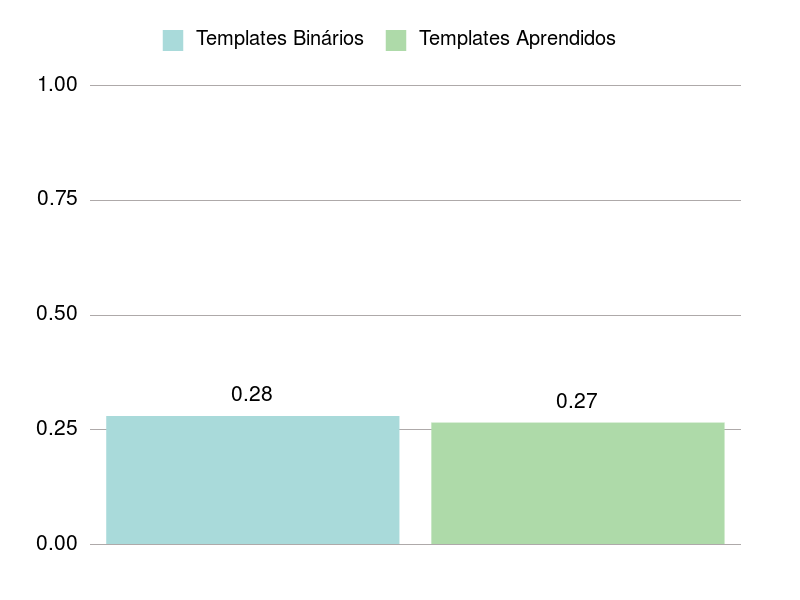
\includegraphics[width=13cm]{figuras/01-templates-binarios-e-aprendidos.png}
            \caption{\label{fig:exp:templates}Precisões médias obtidas com uso de templates binários e aprendidos.}
        
            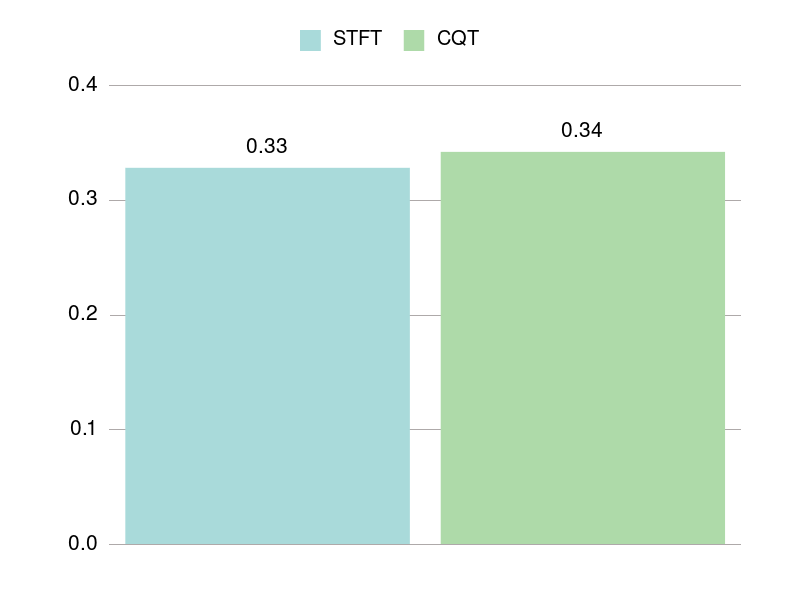
\includegraphics[width=13cm]{figuras/02-stft-e-cqt-com-templates-binarios.png}
            \caption{\label{fig:exp:chroma}Precisões médias obtidas com uso de STFT e CQT para construção do cromagrama.}
        \end{center}
    \end{figure}
    
    \begin{figure}[htb]
        \begin{center}
            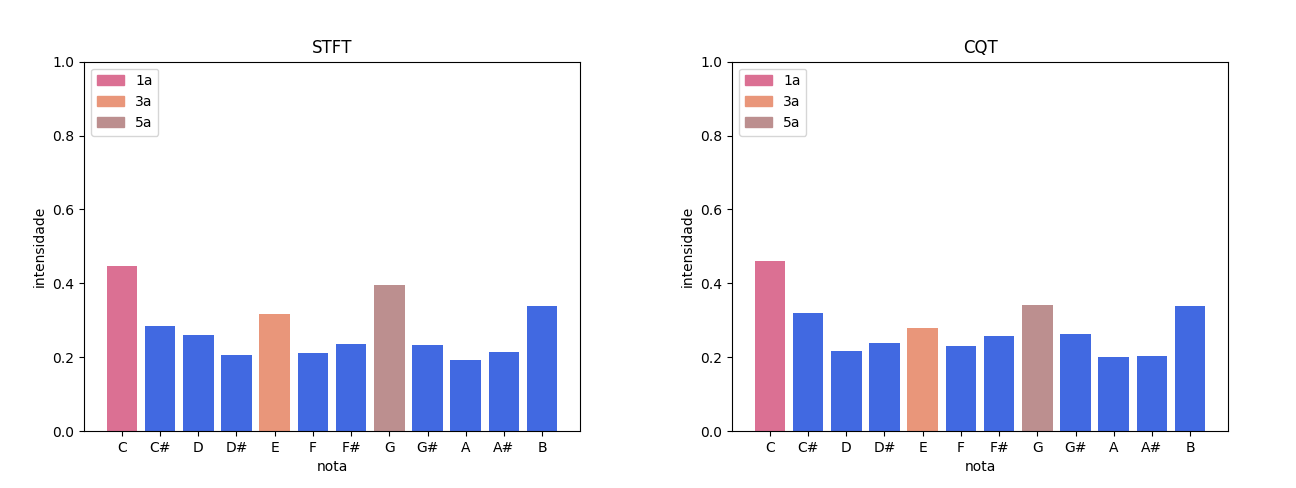
\includegraphics[width=16cm]{figuras/mayor_C.png}
            \caption{\label{fig:exp:template_c}Visualização do cromagrama template construído a partir de cromas STFT e CQT do acorde \textbf{dó maior} (C). As notas marcadas com cores diferentes indicam as notas presentes no acorde. Nota-se que algumas delas possuem menos energia que outras notas, o que se concluiu que acontece por causa da presença de muitos harmônicos nos sinais de áudio usados para treinamento.}
            
            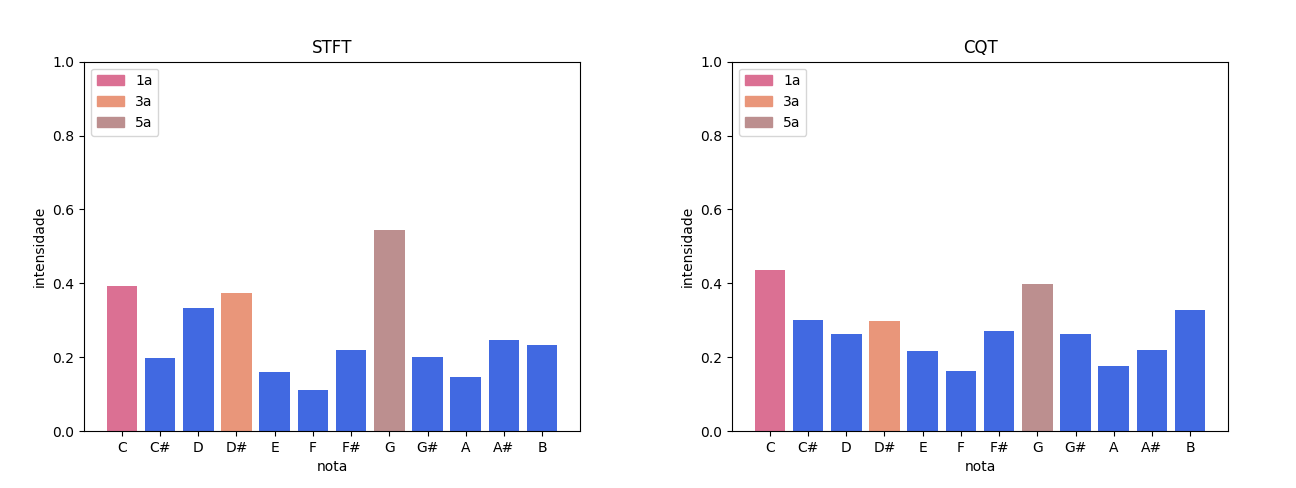
\includegraphics[width=16cm]{figuras/minor_C.png}
            \caption{\label{fig:exp:template_cm}Visualização do cromagrama template construído a partir de cromas STFT e CQT do acorde \textbf{dó menor} (Cm). As notas marcadas com cores diferentes indicam as notas presentes no acorde.}
        \end{center}
    \end{figure}
    
    \begin{figure}[htb]
        \begin{center}
            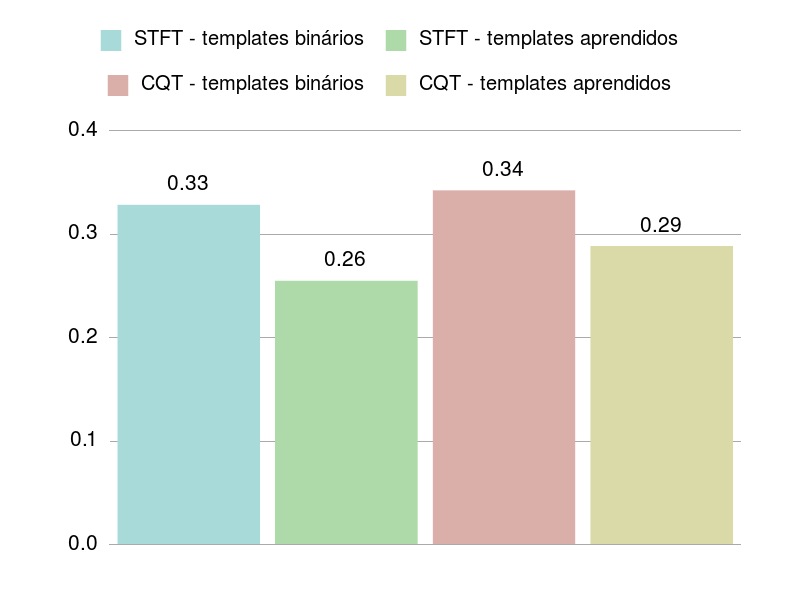
\includegraphics[width=13cm]{figuras/03-stft-e-cqt-templates-bin-e-aprendidos.png}
            \caption{\label{fig:exp:templates_chroma}Comparação entre a precisão média obtida por cromagramas construídos usando STFT, CQT e templates binários e aprendidos.}
            
            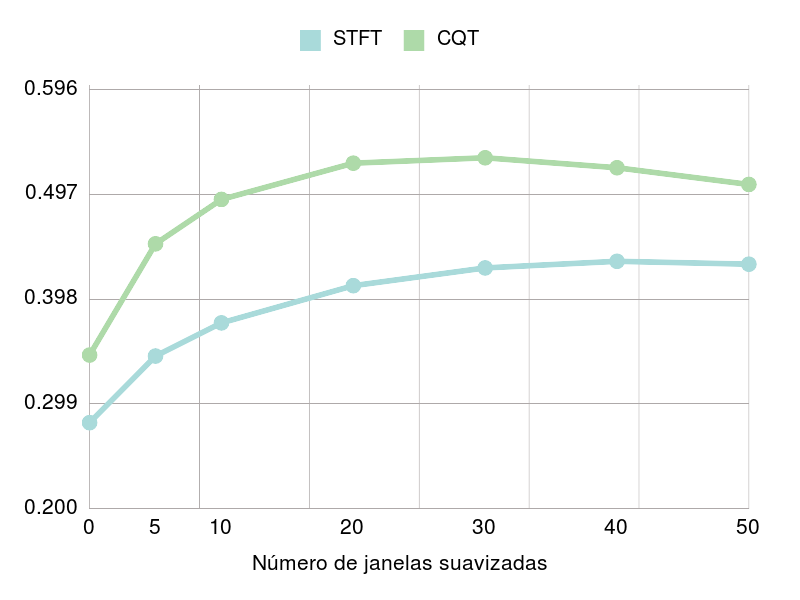
\includegraphics[width=13cm]{figuras/04-stft-e-cqt-bin-suavizacao-temporal.png}
            \caption{\label{fig:exp:temporal}Impacto da suavização temporal com diferentes parâmetros sobre a precisão média do algoritmo.}
        \end{center}
    \end{figure}

    \begin{figure}[htb]
        \begin{center}
            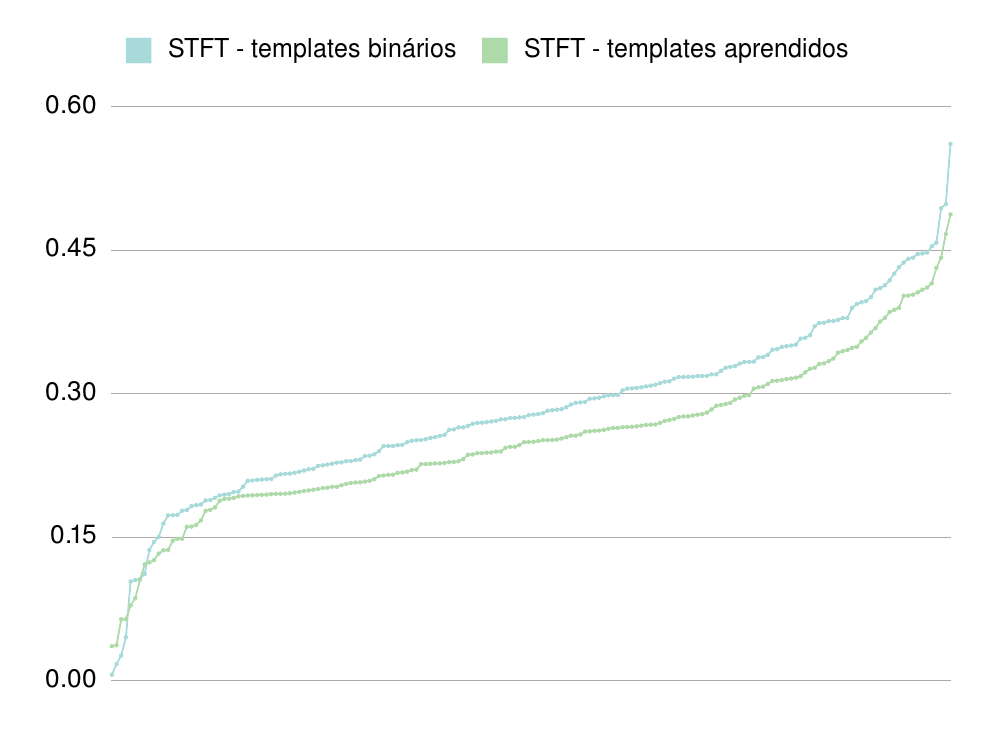
\includegraphics[width=13cm]{figuras/05-distribuicoes-stft-bin-aprendidos.png}
            \caption{\label{fig:exp:dist:stft}Distribuição das precisões obtidas com STFT.}
            
            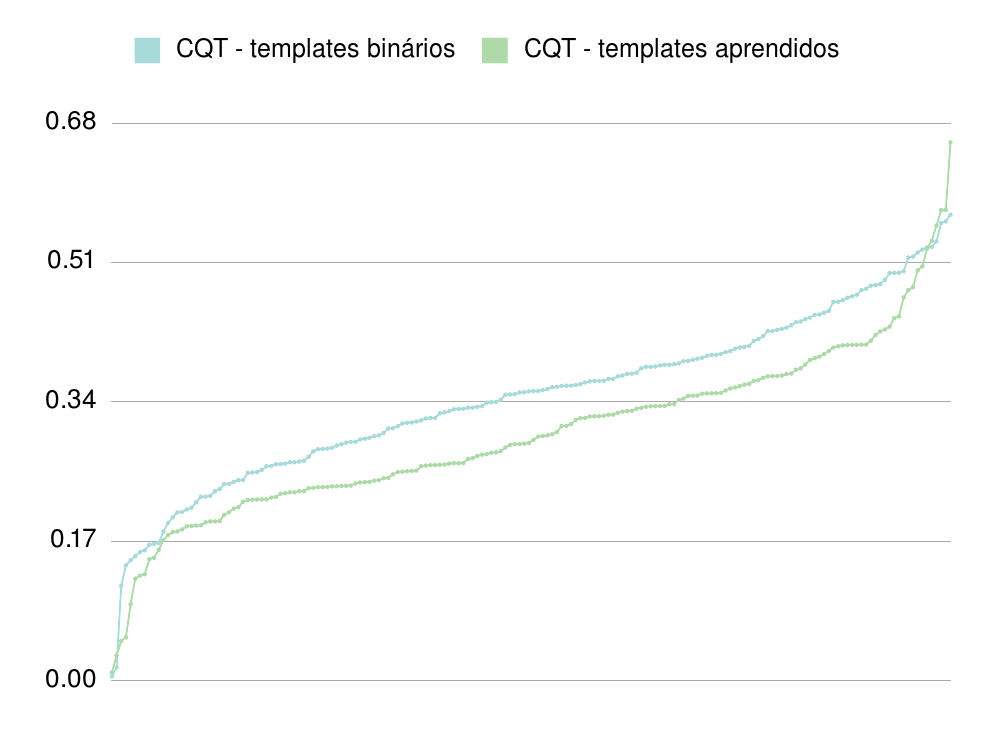
\includegraphics[width=13cm]{figuras/05-distribuicoes-cqt-bin-aprendidos.png}
            \caption{\label{fig:exp:dist:cqt}Distribuição das precisões obtidas com CQT. Observe que as precisões mais baixas estão muito próximas de zero. Esse padrão se repete em todas as parametrizações do algoritmo, o que motivou uma análise caso a caso.}
        \end{center}
    \end{figure}

    \begin{figure}[htb]
        \begin{center}
            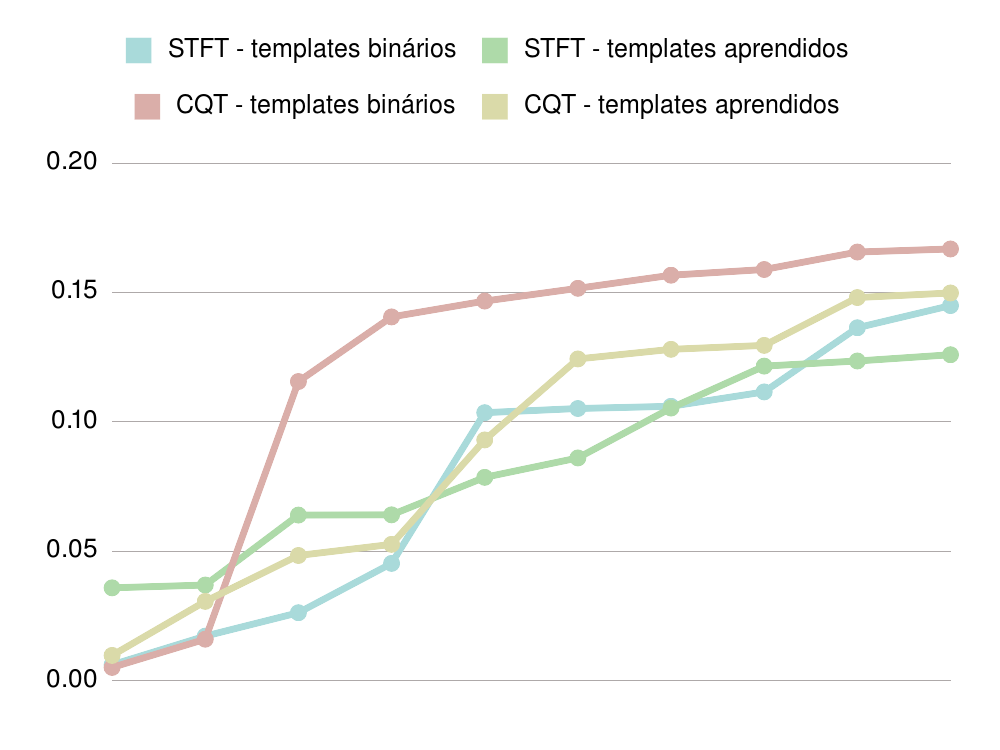
\includegraphics[width=13cm]{figuras/05-distribuicoes-inicial.png}
            \caption{\label{fig:exp:dist:primeiras}Distribuição das 10 piores precisões obtidas com diferentes versões do algoritmo. Nenhuma das técnicas de aperfeiçoamento implementadas nessas versões trouxe uma distribuição mais equilibrada: em todas, se observaram precisões muito próximas de zero.}
            
            
            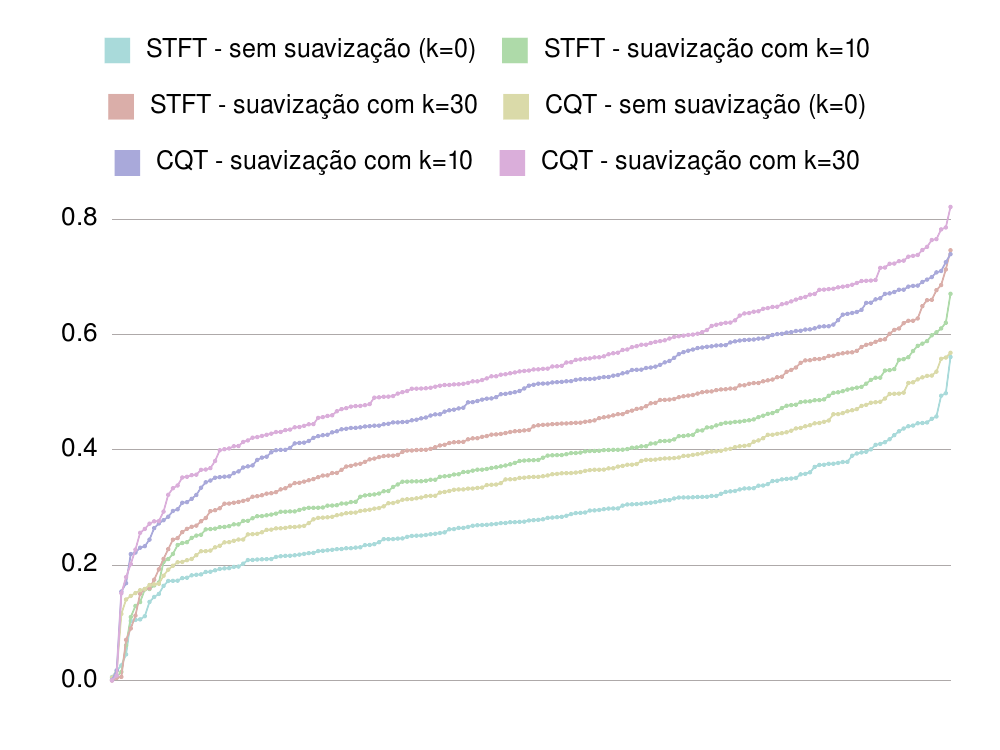
\includegraphics[width=13cm]{figuras/06-distribuicoes-stft-bin-smooth.png}
            \caption{\label{fig:exp:dist:stft_smooth}Impacto da suavização temporal na distribuição das preciões obtidas nos experimentos.}
        \end{center}
    \end{figure}

